\PassOptionsToPackage{unicode=true}{hyperref} % options for packages loaded elsewhere
\PassOptionsToPackage{hyphens}{url}
\documentclass[14pt,ignorenonframetext,compress]{beamer}
\setbeamertemplate{caption}[numbered]
\setbeamertemplate{caption label separator}{: }
\setbeamercolor{caption name}{fg=normal text.fg}
\beamertemplatenavigationsymbolsempty
\usepackage{lmodern}
\usepackage{amssymb,amsmath}
\usepackage{ifxetex,ifluatex}
\usepackage{fixltx2e} % provides \textsubscript
\ifnum 0\ifxetex 1\fi\ifluatex 1\fi=0 % if pdftex
  \usepackage[T1]{fontenc}
  \usepackage[utf8]{inputenc}
\else % if luatex or xelatex
  \ifxetex
    \usepackage{mathspec}
  \else
    \usepackage{fontspec}
\fi
\defaultfontfeatures{Ligatures=TeX,Scale=MatchLowercase}







\fi

  \usetheme[]{monash}



% A default size of 24 is set in beamerthememonash.sty




% use upquote if available, for straight quotes in verbatim environments
\IfFileExists{upquote.sty}{\usepackage{upquote}}{}
% use microtype if available
\IfFileExists{microtype.sty}{%
  \usepackage{microtype}
  \UseMicrotypeSet[protrusion]{basicmath} % disable protrusion for tt fonts
}{}


\newif\ifbibliography


\hypersetup{
      pdftitle={Monash Beamer Class Demonstration},
        pdfauthor={Rob J Hyndman},
          pdfborder={0 0 0},
    breaklinks=true}
%\urlstyle{same}  % Use monospace font for urls




  \usepackage{color}
  \usepackage{fancyvrb}
  \newcommand{\VerbBar}{|}
  \newcommand{\VERB}{\Verb[commandchars=\\\{\}]}
  \DefineVerbatimEnvironment{Highlighting}{Verbatim}{commandchars=\\\{\}}
  % Add ',fontsize=\small' for more characters per line
  \usepackage{framed}
  \definecolor{shadecolor}{RGB}{248,248,248}
  \newenvironment{Shaded}{\begin{snugshade}}{\end{snugshade}}
  \newcommand{\AlertTok}[1]{\textcolor[rgb]{0.94,0.16,0.16}{#1}}
  \newcommand{\AnnotationTok}[1]{\textcolor[rgb]{0.56,0.35,0.01}{\textbf{\textit{#1}}}}
  \newcommand{\AttributeTok}[1]{\textcolor[rgb]{0.77,0.63,0.00}{#1}}
  \newcommand{\BaseNTok}[1]{\textcolor[rgb]{0.00,0.00,0.81}{#1}}
  \newcommand{\BuiltInTok}[1]{#1}
  \newcommand{\CharTok}[1]{\textcolor[rgb]{0.31,0.60,0.02}{#1}}
  \newcommand{\CommentTok}[1]{\textcolor[rgb]{0.56,0.35,0.01}{\textit{#1}}}
  \newcommand{\CommentVarTok}[1]{\textcolor[rgb]{0.56,0.35,0.01}{\textbf{\textit{#1}}}}
  \newcommand{\ConstantTok}[1]{\textcolor[rgb]{0.00,0.00,0.00}{#1}}
  \newcommand{\ControlFlowTok}[1]{\textcolor[rgb]{0.13,0.29,0.53}{\textbf{#1}}}
  \newcommand{\DataTypeTok}[1]{\textcolor[rgb]{0.13,0.29,0.53}{#1}}
  \newcommand{\DecValTok}[1]{\textcolor[rgb]{0.00,0.00,0.81}{#1}}
  \newcommand{\DocumentationTok}[1]{\textcolor[rgb]{0.56,0.35,0.01}{\textbf{\textit{#1}}}}
  \newcommand{\ErrorTok}[1]{\textcolor[rgb]{0.64,0.00,0.00}{\textbf{#1}}}
  \newcommand{\ExtensionTok}[1]{#1}
  \newcommand{\FloatTok}[1]{\textcolor[rgb]{0.00,0.00,0.81}{#1}}
  \newcommand{\FunctionTok}[1]{\textcolor[rgb]{0.00,0.00,0.00}{#1}}
  \newcommand{\ImportTok}[1]{#1}
  \newcommand{\InformationTok}[1]{\textcolor[rgb]{0.56,0.35,0.01}{\textbf{\textit{#1}}}}
  \newcommand{\KeywordTok}[1]{\textcolor[rgb]{0.13,0.29,0.53}{\textbf{#1}}}
  \newcommand{\NormalTok}[1]{#1}
  \newcommand{\OperatorTok}[1]{\textcolor[rgb]{0.81,0.36,0.00}{\textbf{#1}}}
  \newcommand{\OtherTok}[1]{\textcolor[rgb]{0.56,0.35,0.01}{#1}}
  \newcommand{\PreprocessorTok}[1]{\textcolor[rgb]{0.56,0.35,0.01}{\textit{#1}}}
  \newcommand{\RegionMarkerTok}[1]{#1}
  \newcommand{\SpecialCharTok}[1]{\textcolor[rgb]{0.00,0.00,0.00}{#1}}
  \newcommand{\SpecialStringTok}[1]{\textcolor[rgb]{0.31,0.60,0.02}{#1}}
  \newcommand{\StringTok}[1]{\textcolor[rgb]{0.31,0.60,0.02}{#1}}
  \newcommand{\VariableTok}[1]{\textcolor[rgb]{0.00,0.00,0.00}{#1}}
  \newcommand{\VerbatimStringTok}[1]{\textcolor[rgb]{0.31,0.60,0.02}{#1}}
  \newcommand{\WarningTok}[1]{\textcolor[rgb]{0.56,0.35,0.01}{\textbf{\textit{#1}}}}

  \usepackage{longtable,booktabs}
  \usepackage{caption}
  % These lines are needed to make table captions work with longtable:
  \makeatletter
  \def\fnum@table{\tablename~\thetable}
  \makeatother

  \usepackage{graphicx,grffile}
  \makeatletter
  \def\maxwidth{\ifdim\Gin@nat@width>\linewidth\linewidth\else\Gin@nat@width\fi}
  \def\maxheight{\ifdim\Gin@nat@height>\textheight0.8\textheight\else\Gin@nat@height\fi}
  \makeatother
  % Scale images if necessary, so that they will not overflow the page
  % margins by default, and it is still possible to overwrite the defaults
  % using explicit options in \includegraphics[width, height, ...]{}
  \setkeys{Gin}{width=\maxwidth,height=\maxheight,keepaspectratio}

% Prevent slide breaks in the middle of a paragraph:
\widowpenalties 1 10000
\raggedbottom

  \AtBeginPart{
    \let\insertpartnumber\relax
    \let\partname\relax
    \frame{\partpage}
  }
  \AtBeginSection{
    \ifbibliography
    \else
      \let\insertsectionnumber\relax
      \let\sectionname\relax
      \frame{\sectionpage}
    \fi
  }
  \AtBeginSubsection{
    \let\insertsubsectionnumber\relax
    \let\subsectionname\relax
    \frame{\subsectionpage}
  }



\setlength{\parindent}{0pt}
\setlength{\parskip}{6pt plus 2pt minus 1pt}
\setlength{\emergencystretch}{3em}  % prevent overfull lines
\providecommand{\tightlist}{%
  \setlength{\itemsep}{0pt}\setlength{\parskip}{0pt}}

  \setcounter{secnumdepth}{0}



%% Monash overrides
\AtBeginSection[]{
   \frame<beamer>{
   \frametitle{Outline}
   \tableofcontents[currentsection,hideallsubsections]
  }}
% Redefine shaded environment if it exists (to ensure text is black)
\ifcsname Shaded\endcsname
  \definecolor{shadecolor}{RGB}{225,225,225}
  \renewenvironment{Shaded}{\color{black}\begin{snugshade}\color{black}}{\end{snugshade}}
\fi
%%

  \title[]{Monash Beamer Class Demonstration}


  \author[
        Rob J Hyndman
    ]{Rob J Hyndman}


\date[
      \today
  ]{
      \today
        }

\begin{document}

% Hide progress bar and footline on titlepage
  \begin{frame}[plain]
  \titlepage
  \end{frame}


   \frame<beamer>{
   \frametitle{Outline}
   \tableofcontents[hideallsubsections]
  }

\hypertarget{intro}{%
\section{Intro}\label{intro}}

\begin{frame}[fragile]{Slide with bullets}
\protect\hypertarget{slide-with-bullets}{}

\begin{itemize}
\tightlist
\item
  Bullet 1
\item
  Bullet 2
\item
  Bullet 3
\end{itemize}

Use \texttt{\textbackslash{}alert} to \alert{highlight} some text

\begin{block}{Some enumeration}

\begin{enumerate}
\tightlist
\item
  The first item
\item
  Stuff
\item
  Nonsense
\end{enumerate}

\end{block}

\end{frame}

\hypertarget{using-r}{%
\section{Using R}\label{using-r}}

\begin{frame}[fragile]{Slide with R output}
\protect\hypertarget{slide-with-r-output}{}

\begin{Shaded}
\begin{Highlighting}[]
\KeywordTok{summary}\NormalTok{(cars)}
\end{Highlighting}
\end{Shaded}

\begin{verbatim}
##      speed           dist       
##  Min.   : 4.0   Min.   :  2.00  
##  1st Qu.:12.0   1st Qu.: 26.00  
##  Median :15.0   Median : 36.00  
##  Mean   :15.4   Mean   : 42.98  
##  3rd Qu.:19.0   3rd Qu.: 56.00  
##  Max.   :25.0   Max.   :120.00
\end{verbatim}

\end{frame}

\begin{frame}{Slide with graphics}
\protect\hypertarget{slide-with-graphics}{}

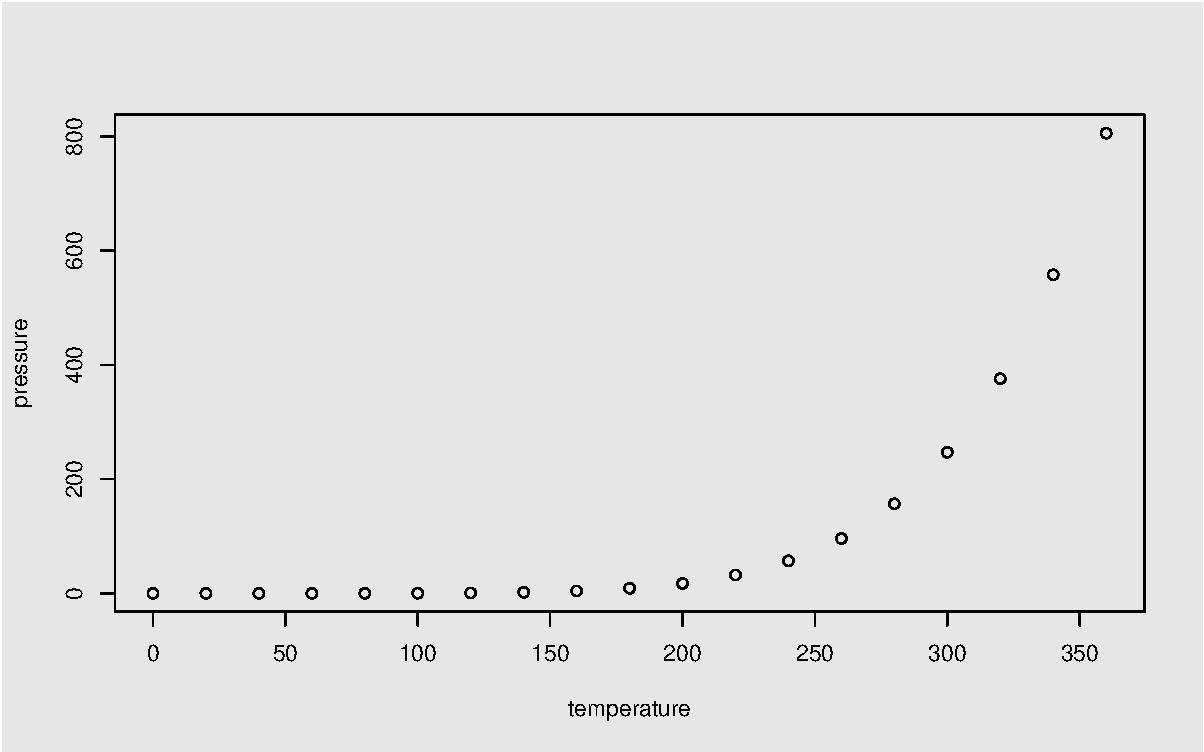
\includegraphics{Introduction_files/figure-beamer/pressure-1.pdf}

\end{frame}

\begin{frame}{Slide with mathematics}
\protect\hypertarget{slide-with-mathematics}{}

Quantile score for observation \(y\). For \(0<p<1\):

\begin{block}{}
  \[
    S(y_t,q_t(p)) = \left\{
      \begin{array}{rl}
            p(y_t-q_t(p)) & \text{if $y_t \ge q_t(p)$}\\
        (1-p)(q_t(p)-y_t) & \text{if $y_t < q_t(p)$}
      \end{array}\right.
  \]
\end{block}

Average score over all percentiles gives the best distribution forecast:
\[
  QS = \frac{1}{99T}\sum_{p=1}^{99}\sum_{t=1}^T S(q_t(p),y_t)
\]

\end{frame}

\hypertarget{rmarkdown-examples}{%
\section{RMarkdown Examples}\label{rmarkdown-examples}}

\begin{frame}[fragile]{R Figure}
\protect\hypertarget{r-figure}{}

The following code generates the plot on the next slide (taken from
\texttt{help(bxp)} and modified slightly):

\small

\begin{Shaded}
\begin{Highlighting}[]
\KeywordTok{library}\NormalTok{(stats)}
\KeywordTok{set.seed}\NormalTok{(}\DecValTok{753}\NormalTok{)}
\NormalTok{bx.p <-}\StringTok{ }\KeywordTok{boxplot}\NormalTok{(}\KeywordTok{split}\NormalTok{(}\KeywordTok{rt}\NormalTok{(}\DecValTok{100}\NormalTok{, }\DecValTok{4}\NormalTok{),}
                      \KeywordTok{gl}\NormalTok{(}\DecValTok{5}\NormalTok{, }\DecValTok{20}\NormalTok{)), }\DataTypeTok{plot=}\OtherTok{FALSE}\NormalTok{)}
\KeywordTok{bxp}\NormalTok{(bx.p, }\DataTypeTok{notch =} \OtherTok{FALSE}\NormalTok{, }\DataTypeTok{boxfill =} \StringTok{"orange"}\NormalTok{,}
    \DataTypeTok{frame =} \OtherTok{FALSE}\NormalTok{, }\DataTypeTok{outl =} \OtherTok{TRUE}\NormalTok{,}
    \DataTypeTok{main =} \StringTok{"Example from help(bxp)"}\NormalTok{)}
\end{Highlighting}
\end{Shaded}

\end{frame}

\begin{frame}{R Figure}
\protect\hypertarget{r-figure-1}{}

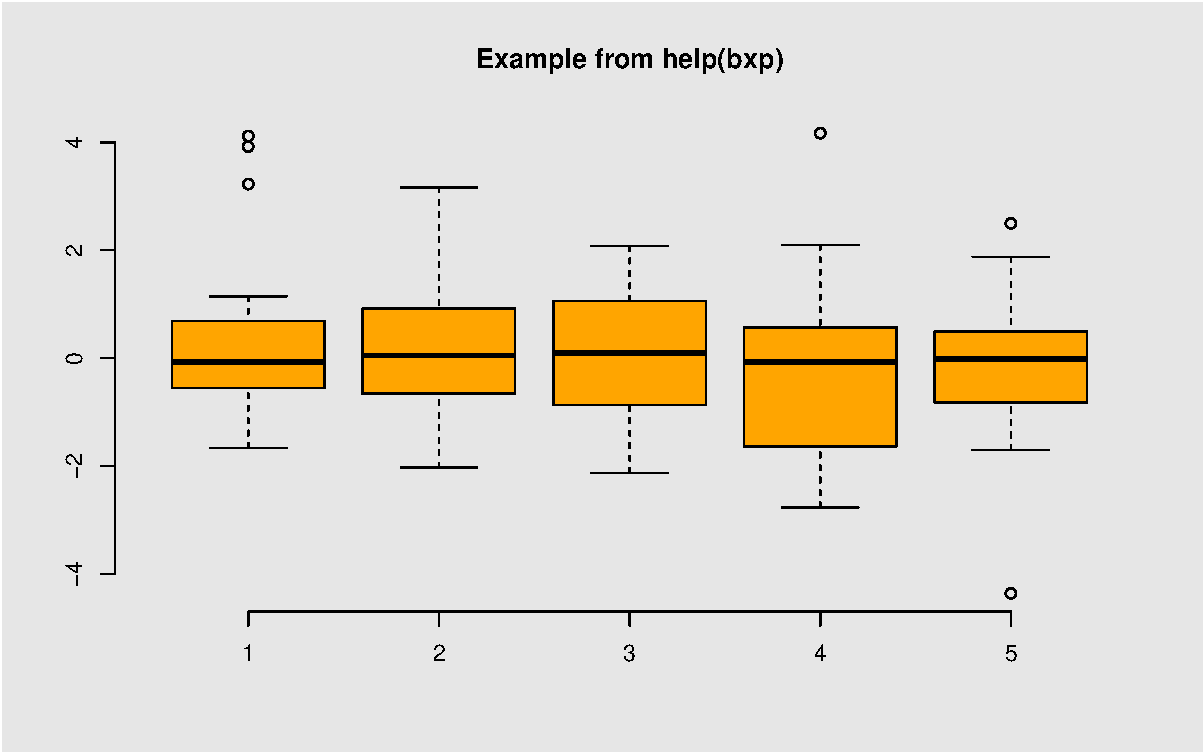
\includegraphics{Introduction_files/figure-beamer/pressureFig-1.pdf}

\end{frame}

\begin{frame}[fragile]{R Table}
\protect\hypertarget{r-table}{}

A simple \texttt{knitr::kable} example:

\small

\begin{Shaded}
\begin{Highlighting}[]
\NormalTok{knitr}\OperatorTok{::}\KeywordTok{kable}\NormalTok{(mtcars[}\DecValTok{1}\OperatorTok{:}\DecValTok{4}\NormalTok{, }\DecValTok{1}\OperatorTok{:}\DecValTok{7}\NormalTok{],}
       \DataTypeTok{caption=}\StringTok{"(Parts of) the mtcars dataset"}\NormalTok{)}
\end{Highlighting}
\end{Shaded}

\begin{longtable}[]{@{}lrrrrrrr@{}}
\caption{(Parts of) the mtcars dataset}\tabularnewline
\toprule
& mpg & cyl & disp & hp & drat & wt & qsec\tabularnewline
\midrule
\endfirsthead
\toprule
& mpg & cyl & disp & hp & drat & wt & qsec\tabularnewline
\midrule
\endhead
Mazda RX4 & 21.0 & 6 & 160 & 110 & 3.90 & 2.620 & 16.46\tabularnewline
Mazda RX4 Wag & 21.0 & 6 & 160 & 110 & 3.90 & 2.875 &
17.02\tabularnewline
Datsun 710 & 22.8 & 4 & 108 & 93 & 3.85 & 2.320 & 18.61\tabularnewline
Hornet 4 Drive & 21.4 & 6 & 258 & 110 & 3.08 & 3.215 &
19.44\tabularnewline
\bottomrule
\end{longtable}

\end{frame}

\begin{frame}{Resources}
\protect\hypertarget{resources}{}

\begin{block}{For more information:}

\begin{itemize}
\tightlist
\item
  See the \href{https://github.com/rstudio/rmarkdown}{RMarkdown
  repository} for more on RMarkdown
\item
  See the \href{https://github.com/eddelbuettel/binb}{binb repository}
  for more on binb
\item
  See the \href{https://github.com/eddelbuettel/binb/vignettes}{binb
  vignettes} for more examples.
\end{itemize}

\end{block}

\end{frame}




\end{document}
